
The reference data for congestion measurement is provided by ASTRA (Bundesamt für Strassen). There are four datasets: 
\begin{itemize}
\item Dataset 1: measurement of 2014 July, 18. - 19.
\item Dataset 2: measurement of 2014 August, first
\item Dataset 3: measurement of 2014 July, 25. - 26.
\item Dataset 4: measurement of 2014 August, second
\end{itemize}

In a first step the model will be trained by dataset 1 and 2. The authors wrote a program which calculates specified values of a specified variable (moveProb and moveCorr) for a given number of times. With other words, it finds the optimal parameter values that minimizes the error of measured congestion. In a second step, the datasets 3 and 4 are used to evaluate the previous trained model.

\subsection{Preparing dataset -- curve fitting}
The timestamps for the measurement are irregular. In order to compare the congestion from the model to the reference data, the breakpoints will be interpolated. The resulting curve can be used to generate regular timestamps for measurement. The authors have decided to go for a linear interpolation. That means that every point will be connected by a straight line with its neighbour, see on the figures below. A linear interpolation is reasonable, because the congestion length between two breakpoints can't change very quickly.

%Die Referenzdaten vom ASTRA (Bundesamt für Strassen) enthalten Staumessungen. Diese sind in unregelmässigen Abständen gemessen. Um einen Vergleich mit der Messung im Modell 
%vorzunehmen, werden die Datenpunkte Interpoliert. Die gefundene Kurve wird dann benutzt, um regelmässige Messungen zu generieren. Die Authoren haben sich für eine lineare %Interpolation entschieden, sodass Punkt zu Punkt mit einer Geraden verbunden wird. Dies ist sinnvoll, weil die Länge des Staus zwischen zwei Punkten nur geringfügig ändern kann.

\begin{figure}[h]\centering
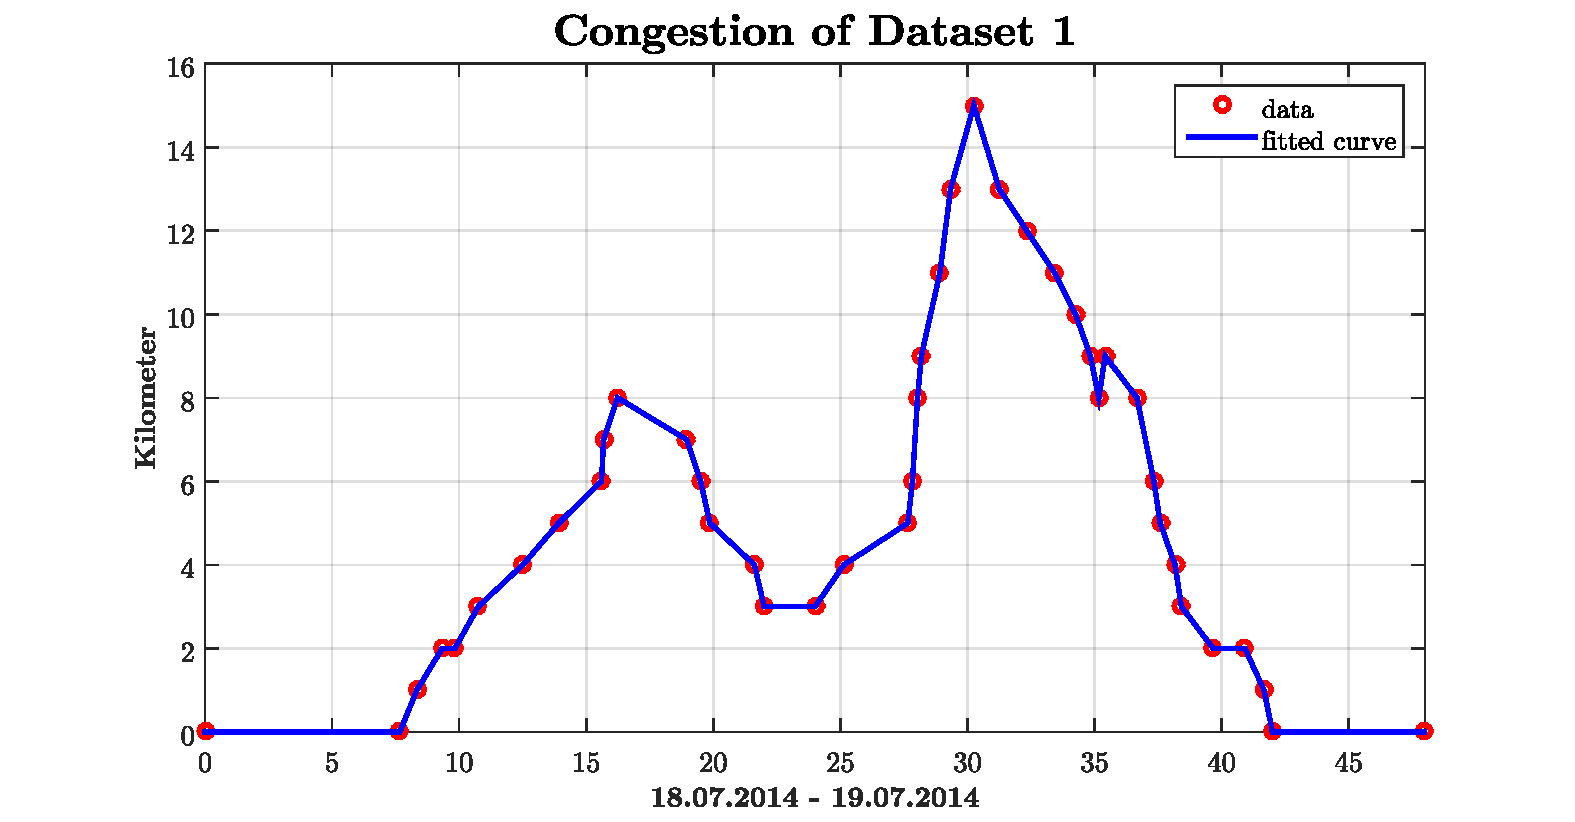
\includegraphics[width=.9\textwidth]{dataset1.pdf}
\caption{Dataset 1}
\end{figure}
\begin{figure}[h]\centering
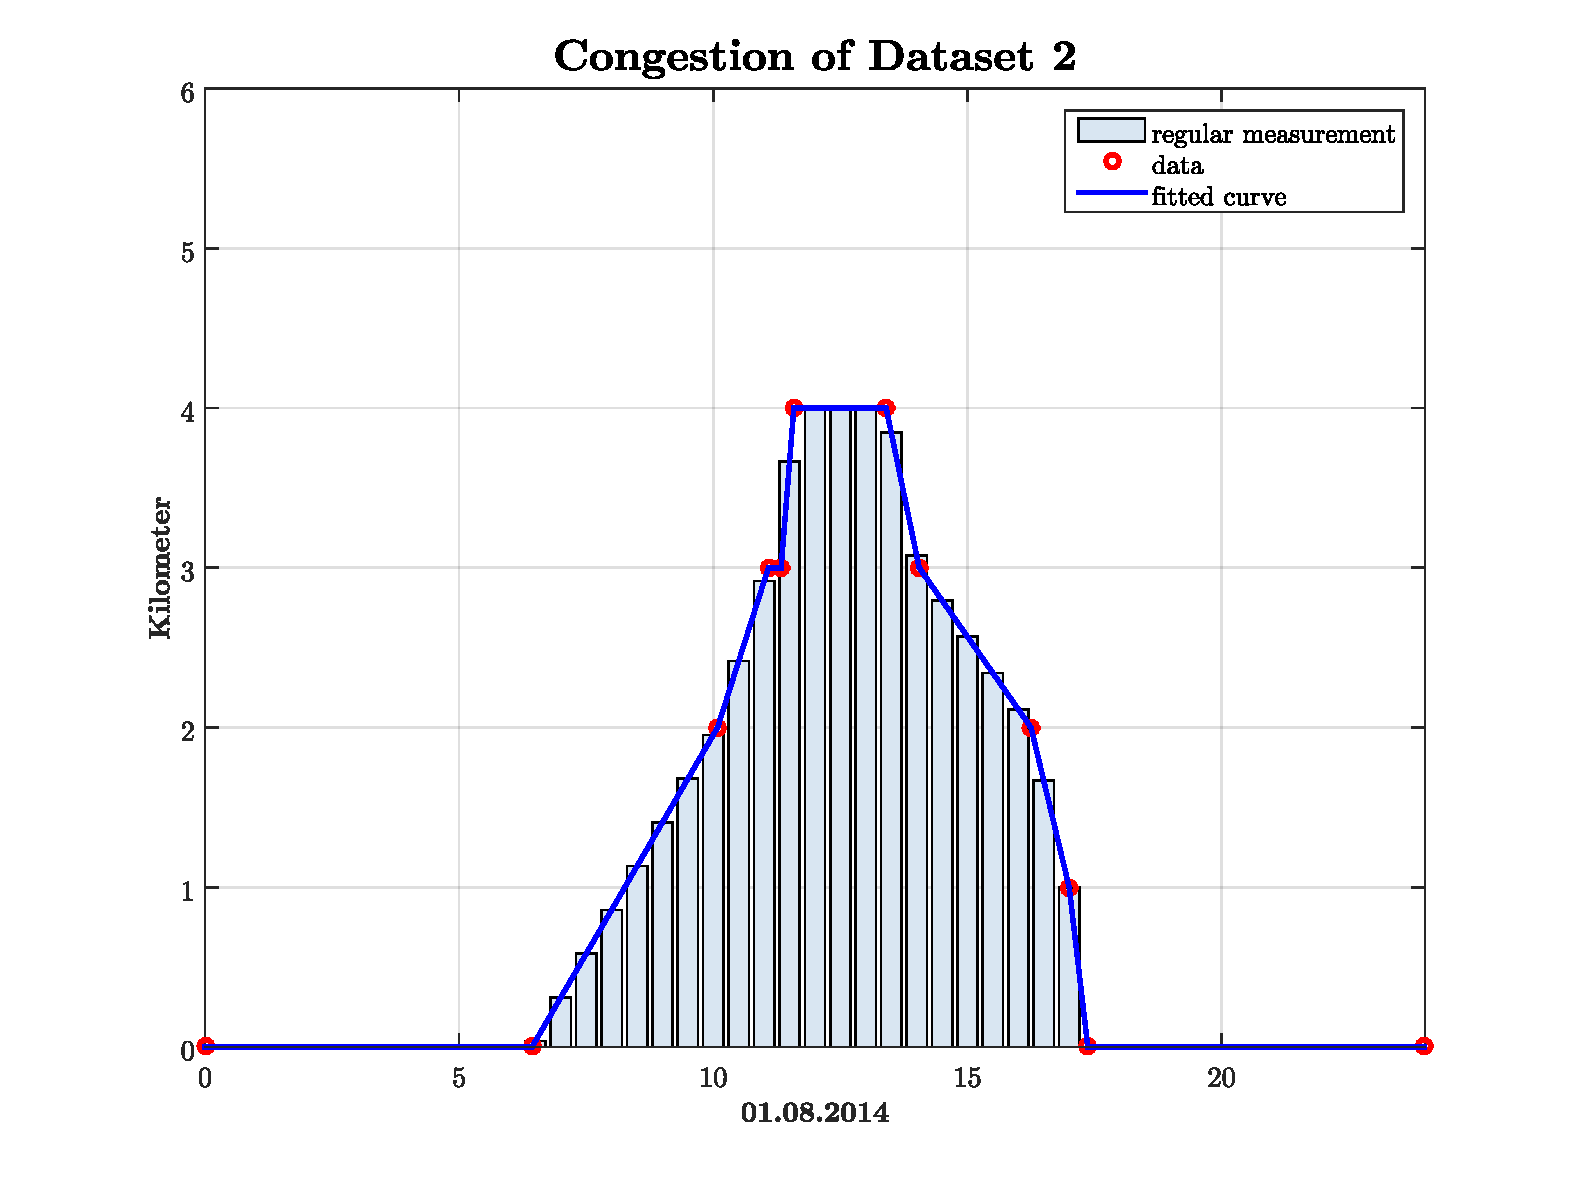
\includegraphics[width=.9\textwidth]{dataset2.pdf}
\caption{Dataset 2, added regular measurements for comparison}
\end{figure}

\subsection{train model}
